\section{Performance Discussion}\label{sec:experiments}

In this section, we use our \ompi and \abft QR implementations to evaluate the
performance of the \cof protocol. We use two test platforms. The first machine,
``Dancer'', is a 16-node cluster. All nodes are equipped with two 2.27GHz
quad-core Intel E5520 CPUs with a 20GB/s Infiniband interconnect. Solid State
Drive (SSD) disks are used as the checkpoint storage media. The second system is
the ``Kraken'' supercomputer. Kraken is a Cray XT5 machine with 9,408 compute
nodes.  Each node has two Istanbul 2.6 GHz six-core AMD Opteron processors, 16
GB of memory, and is connected to other nodes through the SeaStar2+
interconnect. The scalable cluster file system ``Lustre'' is used to store
checkpoints.

\subsection{MPI Library Overhead}

One of the concerns when evaluating the performance of fault tolerance
techniques is the amount of overhead introduced by the fault tolerance
management additions. Our implementation of fault detection and notification is
mostly implemented in the non-critical ORTE runtime. Typical HPC systems feature
a separated service network (usually Ethernet-based) and a performance
interconnect, hence health monitoring traffic, which happens on the OOB service
network, is physically separated from the MPI communications, leaving no
opportunity for network jitter. Changes to MPI functions are minimal: the same
condition that used to trigger unconditional abort has been repurposed to
trigger error handlers. As expected, no impact on MPI bandwidth or latency was
measured.
%(Infiniband and Portals results not shown for lack of space).
The memory usage of the MPI library is slightly increased, as the incarnation
number doubles the size of process names; however, this is negligible in typical
deployments.

\subsection{Failure Detection}\label{sec:experiments:fd}

According to the requirement specified in Section~\ref{sec:interface}, only
in-band failure detection is required to enable \cof. Processes detecting a
failure checkpoint then exit, cascading the failure to processes communicating
with them. However, no recovery action (in particular checkpointing) can take 
place before a failure has been
notified. Thanks to asynchronous failure propagation in the
runtime, responsiveness can be greatly improved, with a high probability for the
next MPI call to detect the failures, regardless of communication pattern or
checkpoint duration.

\begin{figure}[htb]
\centering 
  \subfigure[Linear OOB Routing]{
    \label{fig:linear}
    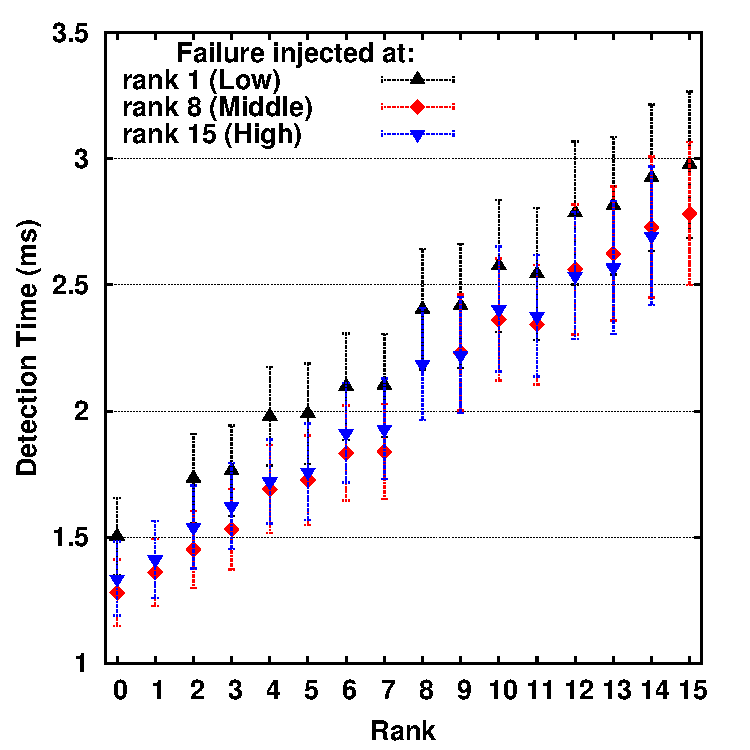
\includegraphics[width=.49\linewidth]{figures/failure_detection_linear_errbars}}
  \hfill
  \subfigure[Binomial OOB Routing]{
    \label{fig:binomial}
    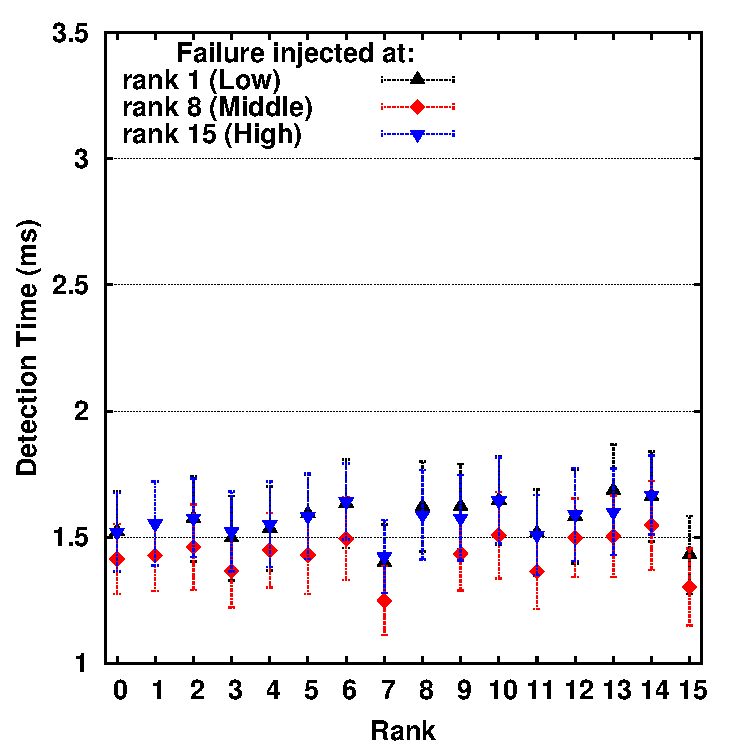
\includegraphics[width=.49\linewidth]{figures/failure_detection_binomial_errbars}}\vspace{-.2cm}
\caption{Failure detection time, sorted by process rank, depending on the OOB overlay network used for 
failure propagation.}\label{fig:detect}
\end{figure}

We designed a micro-benchmark to measure failure detection time as
experienced by MPI processes. The benchmark code synchronizes with an
\mpifunc{MPI\_BARRIER}, stores the reference date, injects a failure at a specific
rank, and enters a ring algorithm until the MPI error handler stores the
detection date. The OOB routing topology used by the ORTE runtime introduces a
non-uniform distance to the failed process, hence failure detection time
experienced by a process may vary depending on both the used OOB 
overlay topology and the position of the failed
process in the topology. Figure~\ref{fig:linear}
and~\ref{fig:binomial} present the case of the linear and
binomial OOB topologies, respectively. The curves ``Low, Middle, High'' present the
behavior for failures happening at different positions in the OOB
topology. On the horizontal axis is the rank of the detecting process,
on the vertical axis is the detection time it experienced. The
experiment uses 16 nodes, with one process per node, MPI over Infiniband, OOB
over Ethernet, an average of 20 runs, and the MPI barrier latency is four orders of
magnitude lower than measured values.

In the linear topology (Figure~\ref{fig:linear}) every runtime process
is connected to the \emph{mpirun} process. For a higher rank, failure
detection time increases linearly because it is notified by the
\emph{mpirun} process only after the notification has been sent to all
lower ranks. This issue is bound to increase with scale. The binomial
tree topology (Figure~\ref{fig:binomial}) exhibits a similar best
failure detection time. However, this more scalable topology has a low
output degree and eliminates most contentions on outgoing messages,
resulting in a more stable, lower average detection time, regardless of the
failure position. Overall, failure detection time is on the order of
milliseconds, a much smaller figure than typical checkpoint time.

% WE SHOULD HAVE SOME RESULTS WITH AUTO-FT AND/OR APP BASED PERIODIC CHECKPOINT


%
%\begin{figure}[thb]
%\centering
%\begin{minipage}[t]{.29\linewidth}
%	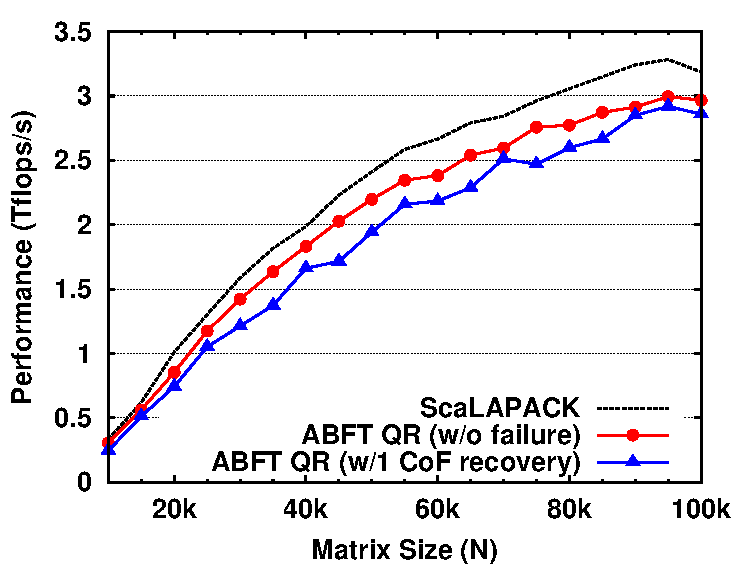
\includegraphics[width=\linewidth]{figures/kraken_new_data}
%	\vspace{-.6cm}\caption{ABFT QR and one \cof recovery on Kraken (Lustre).}%($24\times 24$ grid)
%	\label{fig:kraken_performance}	
%\end{minipage}
%\hfill
%\begin{minipage}[t]{.29\linewidth}
%    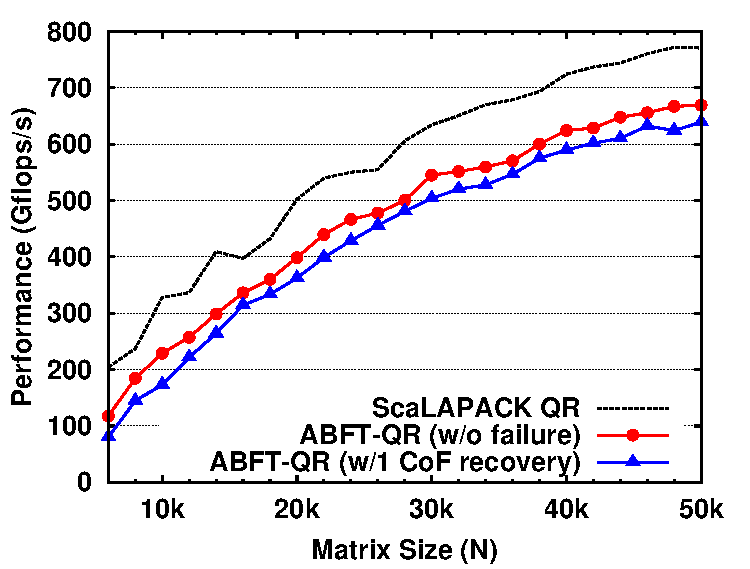
\includegraphics[width=\linewidth]{figures/dancer_performance_data}
%	\vspace{-.6cm}\caption{ABFT QR and one \cof recovery on Dancer (local SSD).} %($16\times 8$ grid)
%    \label{fig:dancer_performance}
%\end{minipage}
%\hfill
%\begin{minipage}[t]{.29\linewidth}
%    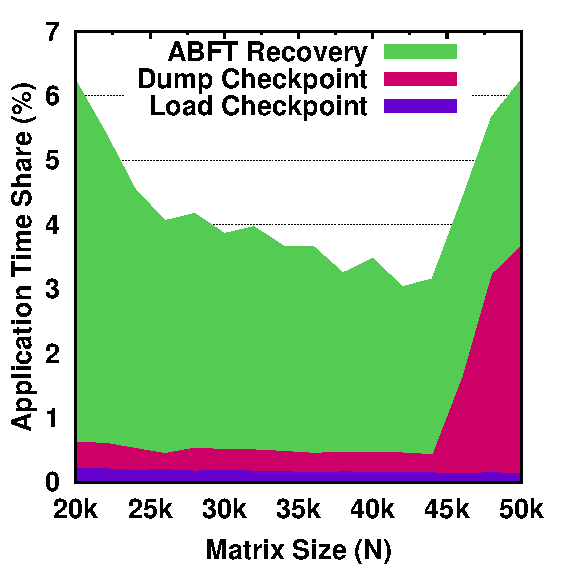
\includegraphics[width=\linewidth]{figures/dancer_1_error_timing_process_new_data}
%	\vspace{-.6cm}\caption{Time breakdown of one \cof recovery on Dancer (local SSD).}
%    \label{fig:dancer_timing}
%\end{minipage}\vspace{-.3cm}
%\end{figure}

\begin{figure}[thb]
\centering
	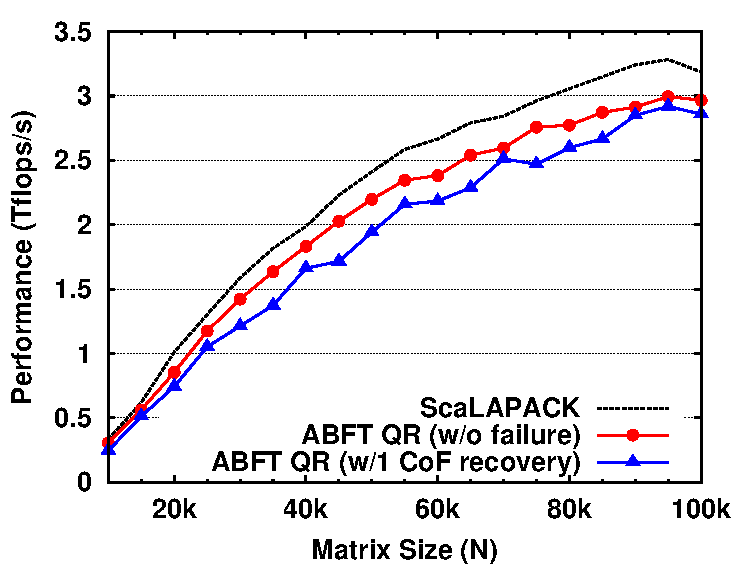
\includegraphics[scale=.6]{figures/kraken_new_data}
	%\vspace{-.6cm}
	\caption{ABFT QR and one \cof recovery on Kraken (Lustre).}%($24\times 24$ grid)
	\label{fig:kraken_performance}	
\end{figure}

\subsection{Checkpoint-on-Failure QR Performance}

\paragraph*{Supercomputer Performance:}
Figure~\ref{fig:kraken_performance} presents the performance on the
Kraken supercomputer. The process grid is $24\times 24$ and the block size
is 100. \abft-QR (no failure) presents the performance of the \cof QR
implementation, in a fault-free execution; it is noteworthy, that when
there are no failures, the performance is exactly identical to the
performance of the unmodified \abft-QR implementation. The \abft-QR (with
\cof recovery, latter called \cof-QR for brevity) curves present the performance when a failure is injected after
the first step of the PDLARFB kernel. The performance of the non-fault
tolerant ScaLAPACK QR is also presented for reference.

Without failures, the performance overhead compared to the regular
ScaLAPACK is caused by the extra computation to maintain the checksums inherent to the \abft
algorithm~\cite{pengduppopp12}; this extra computation is unchanged 
when applying the \cof method to the \abft-QR. 
Only on runs where failures occur does the \cof protocol
undergoe the supplementary overhead of storing and reloading
checkpoints. However, the performance of \cof-QR remains very
close to the no-failure case. For instance, at matrix size N=100,000,
\cof-QR still achieves 2.86 Tflop/s after recovering from a failure,
which is 90\% of the performance of the non-fault tolerant ScaLAPACK QR.
This demonstrates that the \cof protocol enables efficient, practical
recovery schemes on supercomputers.


\begin{figure}[thb]
\centering
\subfigure[Performance]{
    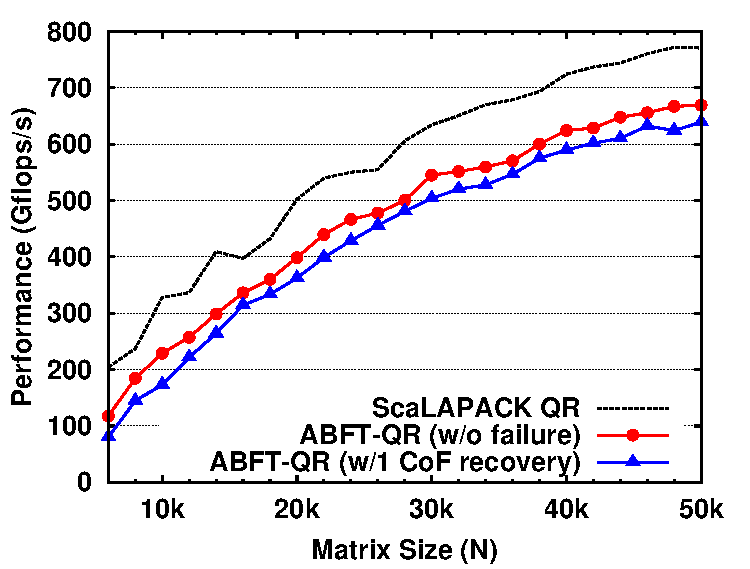
\includegraphics[scale=.6]{figures/dancer_performance_data}
	%\vspace{-.6cm}
    \label{fig:dancer_performance}
}
\hfill
\subfigure[Time breakdown of one \cof recovery]{
    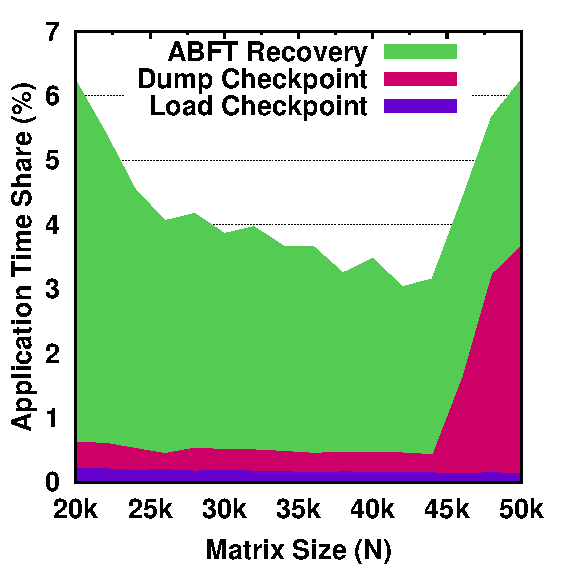
\includegraphics[scale=.6]{figures/dancer_1_error_timing_process_new_data}
	%\vspace{-.6cm}
    \label{fig:dancer_timing}
}
\caption{ABFT QR and one \cof recovery on Dancer (local SSD).}
\end{figure}


\paragraph*{Impact of Local Checkpoint Storage:}

Figure~\ref{fig:dancer_performance} presents the performance of the \cof-QR 
implementation on the Dancer cluster with a $8\times 16$ process
grid. Although a smaller test platform, the Dancer cluster features
local storage on nodes and a variety of performance analysis tools
unavailable on Kraken. As expected (see~\cite{pengduppopp12}), the \abft
method has a higher relative cost on this smaller machine (with a 
smaller number of processors and a smaller problem size, the cost in 
supplementary operations to update checksums is relatively larger). 
Compared to
the Kraken platform, the relative cost of \cof failure recovery is
smaller on Dancer. The \cof protocol incurs disk accesses to store and
load checkpoints when a failure hits, hence the recovery overhead
depends on I/O performance. By breaking down the relative cost of each
recovery step in \cof, Figure~\ref{fig:dancer_timing} shows that
checkpoint saving and loading only takes a small percentage of the total
run-time, thanks to the availability of solid state disks on every node.
Since checkpoint reloading immediately follows checkpointing, the OS
cache satisfies most disk accesses, resulting in high I/O performance. For
matrices larger than N=44,000, the memory usage on each node is high and
decrease the available space for disk cache, explaining the decline in
I/O performance and the higher cost of checkpoint management. Overall,
the presence of fast local storage can be leveraged by the \cof protocol
to speedup recovery (unlike periodic checkpointing, which
depends on remote storage by construction). Nonetheless, as demonstrated by the
efficiency on Kraken, while this is a valuable optimization, it is not a
mandatory requirement for satisfactory performance.

%On a problem of this size, the additional overheads
%are dominated by the time it takes to terminate the failing MPI
%application and relaunch a new one. 


\begin{figure}[thb]
\centering
	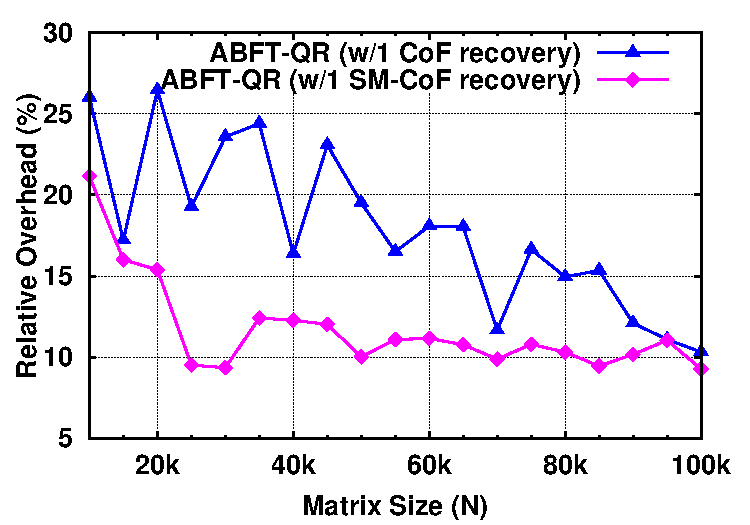
\includegraphics[scale=.6]{figures/kraken_shmem_576cores_squeeze.pdf}
	%\vspace{-.6cm}
	\caption{\abft QR and one recovery on Kraken: comparing
          \cof and SM-\cof overheads.}%($24\times 24$ grid)
	\label{fig:smcof}	
\end{figure}

\paragraph*{Checkpoint-on-Failure, without the Checkpoints:} An
interesting optimization to \cof is to avoid the checkpointing cost
by using the SM-\cof approach described in
Section~\ref{section:application}. In this paragraph, we present the
performance of the QR factorization, when applied by a fragile helper
MPI application, onto a dataset exported through a shared memory
segment from a resilient, non-MPI application. Figure~\ref{fig:smcof}
compares the overhead incurred by introducing a failure with
checkpoint-based \cof recovery versus a shared-memory-\cof recovery
where a master application maintains the dataset resident in memory.

%%%%Not shown in the relative figure, but interesting result anyway
%A first interesting result is that running 
%the non fault tolerant Scalapack QR on the shared memory segment exported
%data does not incur supplementary overhead. 

The cost of the \abft recovery is unchanged by the use of SM-\cof; the
obvious consequence is that, for very small matrix sizes, when the
relative cost of \abft checksum inversion represents a large portion of
the overall compute time, the difference between the shared-memory
optimization and the checkpoint based \cof is small. A similar result is
observed for very large matrices: for a matrix of size $N$,
checkpointing time is $O(N^2)$ while compute time is $O(N^3)$, thus 
the cost of storing and reloading checkpoints is dwarfed by the total 
execution time of the application and achieve similar asymptotic 
performance. 
%%%% I think this explanation is incorrect. ABFT checksum inversion is O(N^2) also, so its moot. 
% As this experiment, intended to understand the cost of a single \cof
%recovery, neglects the fact that since the runtime increases with $N$, so
%is the probability that multiple recoveries are necessary in a
%production run. Unlike the \abft part of the recovery whose overhead 
%decrease with 
For intermediate matrix sizes, however, the cost of checkpointing
represents a significant share of the overhead experienced by the
application during the recovery procedure. In that case, which is the
most relevant in production deployments, the SM-\cof optimization
successfully suppresses the checkpoint overhead and performs similarly to
\abft-QR on a fully fault tolerant MPI implementation, although at the
expense of more complexity in the application code.

